%!TEX root = ../diplomarbeit.tex

\subsection{Technical Issues Concerning Graphics Processing Units}
\label{sec:gpu_technical_issues}

\paragraph{Driver Issue Concerning \texttt{isnan}}
With some GPUs or GPU drivers, basic functions like `bool isnan(float a)` may have bugs and may not always return the expected results. These kind of issues are especially hard to track down because they do not show up in unit tests when running the tests on a different architecture, for example on the local CPU. They also don't raise exceptions.

In this case, the workaround has been to use a custom implementation of the `isnan` function that uses another basic operator to determine the result and circumvents the native implementation of `isnan`.

\begin{ccode}
// Fixed custom replacement of `isnan`:
bool my_is_nan(floating_t a) { return (a != a); }
\end{ccode}

\docpar{The issue is documented in \issue{14}. The workaround is documented in \issue{16}.}


\paragraph{Driver Issue Concerning Kernel Caching}
When changing the kernel code has no effect when running the simulation again, this could be due to a caching issue: The cache for kernels that are included using the `#include` pre-processor statement is not reset automatically when the included files change.

The workaround is to disable caching using an environment variable, or to reset the cache by hand.

\begin{bash}
# Disable caching globally. Despite the name this also works with OpenCL.
export CUDA_CACHE_DISABLE=1

# Reset cache manually:
rm -r ~/.nv/ComputeCache
\end{bash}

\docpar{This problem and the workaround are documented in \issue{15}.}


\paragraph{Numerical Inconsistencies}
Computations that are mathematically equivalent are not guaranteed to be numerically equivalent as well. Performing the same calculation using different formula, or calculating the same quantity using two different, but mathematically equivalent algorithms, may lead to different results.

If such two calculations are performed within one algorithm, this may lead to meaningless results or simulation crashes.

For example, one part of the hole-ice-correction algorithm used the \noun{Pythagorean Theorem} to calculate the distance of the photon from the hole-ice center. Comparing this to the hole-ice radius, the algorithm decided whether the photon is within or outside the cylinder. Another part of the algorithm calculated intersections of the photon trajectory with the hole-ice cylinder. Evaluating the scale parameters $s_1$ and $s_2$ (see figure \ref{fig:aeQuae2U} a), the algorithm decided again whether the photon is within or outside the hole ice.

If the photon is near the hole-ice radius, one mechanism may come to the conclusion that the photon is within the hole-ice cylinder while the other mechanism considers the photon outisde the cylinder. If both mechanisms are used in the same algorithm, this leads to inconsistencies.

The soluation to this problem is to only use one way to determine whether the photon is within or outside the cylinder. The decision may still be ``wrong'' compared to a high-precision calculation, but it will be consistent and not cause the program to crash.

\begin{figure}[htbp]
  \subcaptionbox{using scalar quantities}{\halfimage{intersection-Kahm4UeY}}
  \subcaptionbox{using vectorial quantities}{\halfimage{intersection-vectorial-auloLai2}}
  \caption{Calculating intersections of photon trajectory $AB$ and the hole-ice cylinder represented as circle.}
  \label{fig:aeQuae2U}
\end{figure}


Another, less destructive, but even more demonstrative example for numerical inconsistencies is comparing two ways of calculating intersections as shown in figure \ref{fig:aeQuae2U}.

Both methods are described in section \ref{sec:intersections}. The important difference is that one method uses scalar quantities to calculate the intersection points, the other method uses vectorial quantities and native vector operations. While both methods are mathematically equivalent, their results differ in their numerical precisions, which is visualized in figure \ref{fig:usie5Ohj}: Both simulations show photons hitting an instantly absorbing cylinder. While native vector operations cut the photons cleanly at the cylinder border, using only scalar quantities shows a scraggy border.

\begin{figure}[htbp]
  \subcaptionbox{using scalar quantities to calculate the intersection points coordinate-wise}{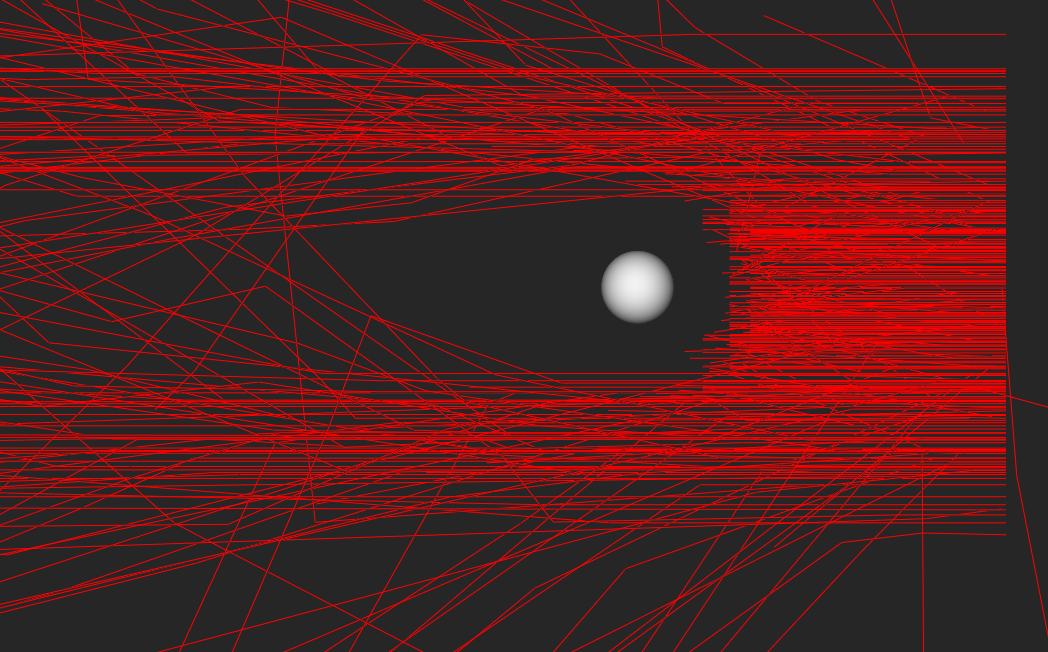
\includegraphics[width=0.48\textwidth, clip, trim = {0 2cm 0 0}]{img/instant-absorption-steamshovel-unclean-usie5Ohj}}\hfill
  \subcaptionbox{using native vector operations to calculate the intersection points}{\halfimage{instant-absorption-steamshovel-moo9Eiqu}}\hfill
  \caption{Simulation of photons propagating towards a cylinder configured for instant absorption. Both simulations are the same except for the method how intersections of photon rays and cylinders are calculated. Using native vector operations (b) leads to numerically more precise results.}
  \label{fig:usie5Ohj}
\end{figure}

\docpar{This issue is documented in \issue{28}.}


\paragraph{Memory Issues: ``OpenCL worker thread died unexpectedly''}
While the user might wholeheartedly agree that the crash is rather unexpected, the error message does not help to find the underlaying issue, which is most probably a memory issue, for example allocating too few or too much memory on the GPU.

To circumvent this issue, this study adds the propagation configuration parameter `MaxNumOutputPhotonsCorrectionFactor` to clsim, which acts as a factor within the calculation that determines how much memory will be allocated for storing photons.

As a rule of thumb, using values from `MaxNumOutputPhotonsCorrectionFactor = 0.1` to `MaxNumOutputPhotonsCorrectionFactor = 1e-3` may resolve the issue. But the memory might then be insufficient to store all propagated photons, especially when photon paths are to be saved as well as compared to only the hits.

Another workaround when creating visualizations is to propagate less photons and/or run the simulation on a CPU. The memory is much larger when running on a CPU such that this issue might not occur on the CPU. But the simulation time will be longer on the CPU.

\docpar{This issue is documented in \issue{23}.}

